\section{Aprendizaje profundo}

Esta Sección introduce en los temas principales del aprendizaje profundo que sirven como base para comprender como funcionan.

\subsection{Redes neuronales}

Una red neuronal se llama así porque pretende modelar el cerebro en código informático. El objetivo final es crear una “inteligencia general artificial”, en otras palabras, un programa que puede aprender todo lo que una persona podría aprender.

Las redes neuronales artificiales son una clase de algoritmos de aprendizaje máquina que aprenden de los datos y se especializan en el reconocimiento de patrones (\cite{rosebrock2017deep}).

Una red neuronal es una función flexible que adapta de manera autónoma su comportamiento para satisfacer la relación entre las entradas y los resultados esperados; por lo que se lee ha denominado como un aproximador universal (\cite{goyal2018Deep}).

\subsection{Perceptrón}

\citeauthor{rosenblatt1958Perceptron} publicó el algoritmo seminal Perceptrón: este modelo es capaz de aprender automáticamente los pesos necesarios para clasificar una entrada.

Perceptrón toma $n$ entradas y produce una única salida binaria si la suma es mayor que el valor de activación. Se dice que la neurona se “dispara” siempre que se excede el valor de activación y se comporta como una función escalonada, lo cual se muestra en la Ecuación \ref{eq:fnStep} (\cite{goyal2018Deep}).

\begin{equation}
\label{eq:fnStep}
    f\left(x\right)=\begin{cases}0 & x -u < 0\\1 & x -u >= 0\end{cases}
\end{equation}



\citeauthor{minsky1969Perceptrons} demostraron que un perceptrón con una función de activación lineal es simplemente un clasificador lineal, incapaz de resolver problemas no lineales (\cite{rosebrock2017deep}). El ejemplo de un problema no lineal es el conjunto de datos XOR Figura \ref{fig:xor}. Esta limitante provoca una disminución en el interés por el modelo Perceptrón.

Perceptrón se puede convertir fácilmente en un algoritmo lineal que procesa un flujo de ejemplos, actualizando el vector de peso solo si el último ejemplo recibido está mal clasificado. Se garantiza que el perceptrón convergerá en una solución si los datos de entrenamiento son linealmente separables, pero de lo contrario no convergerán(\cite{flach2012Machine}).

\begin{figure}[H]
    \centering
    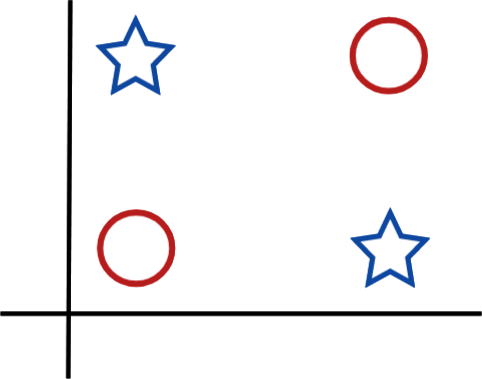
\includegraphics[width=0.5\textwidth]{MarcoTeorico/imgs/XOR.png}
    \caption{Problema XOR, no es linealmente separable.}
    \label{fig:xor}
\end{figure}


\subsection{Redes Neuronales Multicapa}


Al encontrar que el modelo Perceptrón solo puede resolver problemas lineales las investigaciones para esta área disminuyeron considerablemente, sin embargo, \citeauthor{rumelhart1986Parallel} encontraron que este problema puede ser resuelto al unir múltiples perceptrones uno detrás del otro en diferentes combinaciones.

Los perceptrones multicapa o MLP (\textit{Multilayer Perceptron}) son una red neuronal de propagación hacia adelante y se componen de múltiples perceptrones conectados entre sí y que operan en funciones de activación distintivas para permitir mejores mecanismos de aprendizaje. La arquitectura perceptrón multicapa cuenta como mínimo con tres capas: una capa de entrada, una o más capas ocultas y una capa de salida (\cite{swamynathan2017Mastering}) Figura \ref{fig:mlp}.

\begin{figure}[H]
    \centering
    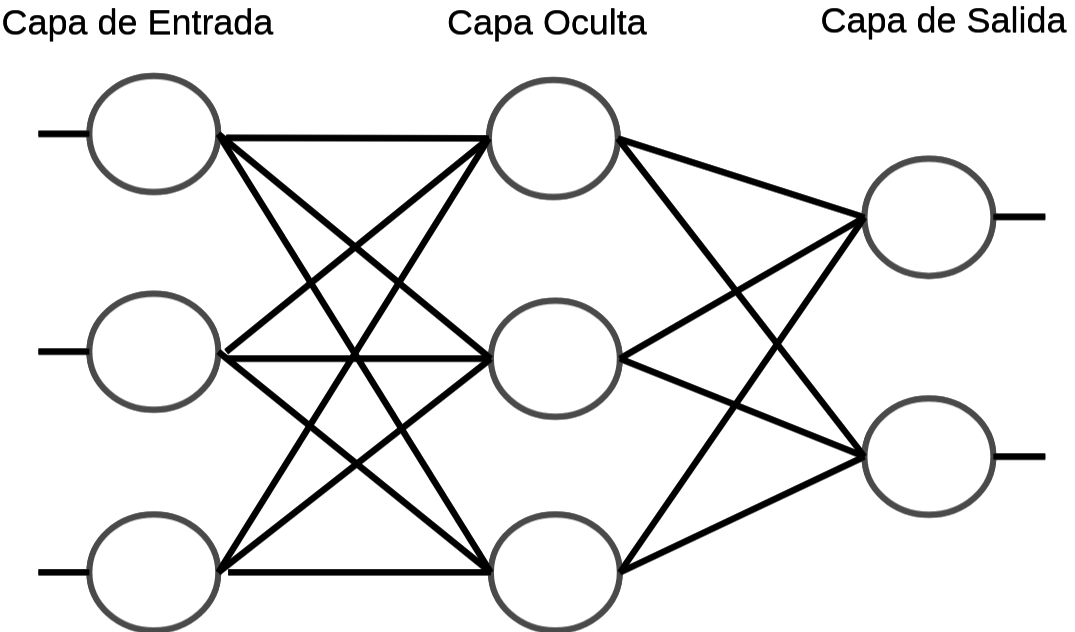
\includegraphics[width=0.5\textwidth]{MarcoTeorico/imgs/MLP.png}
    \caption{Representación básica de red neuronal multicapa.}
    \label{fig:mlp}
\end{figure}

Los MLP también se conocen como aproximadores universales, ya que pueden encontrar la relación entre los valores de entrada y los objetivos, utilizando una cantidad suficiente de neuronas en la capa oculta, alterando los pesos o utilizando datos de entrenamiento adicionales para aproximar la función dada hasta cualquier nivel de precisión. A menudo, con el grado de libertad dado a un MLP, puede superar a la red MLP básica, introduciendo más capas ocultas, con menos neuronas en cada una de las capas ocultas y pesos óptimos. Esto ayuda en el proceso de generalización del modelo (\cite{goyal2018Deep}).

\subsection{Propagación hacia atrás (Backpropagation)}

En las redes neuronales es complicado ajustar sus pesos de entrenamiento por la gran cantidad de conexiones y sus múltiples niveles. Para lograr esta tarea, se utiliza el algoritmo de propagación hacia atrás, creado por \citeauthor{rumelhart1986Parallel} en \citeyear{rumelhart1986Parallel}.

En el algoritmo propagación hacia atrás se calcula qué tan rápido cambia el error a medida que cambia una capa oculta. A partir de ahí, se puede averiguar qué tan rápido cambia el error cuando varia el peso de una conexión individual. Básicamente, pretende encontrar el camino de descenso más pronunciado. Se comienza calculando las derivadas del error con respecto a un solo ejemplo de entrenamiento. Una vez que se tienen las derivadas de error para una capa de unidades ocultas, se utilizan para calcular las derivadas de error para las unidades de la capa siguiente. Y una vez que se encuentran las derivadas del error para las actividades de las unidades ocultas, es bastante fácil obtener las derivadas del error para los pesos que conducen a una unidad oculta (\cite{buduma2017Fundamentals}).

En resumen, el algoritmo de propagación hacia atrás consiste en dos pasos como muestra la Figura \ref{fig:backpropagation}:

\begin{itemize}
\item Propagación hacia adelante: Se calculan los pesos de cada una de las neuronas, desde la capa de entrada hasta la capa de salida.

\item Propagación hacia atrás: Se calcula el error y se actualizan los pesos, desde la capa de salida hasta la capa de entrada.
\end{itemize}

\begin{figure}[H]
    \centering
    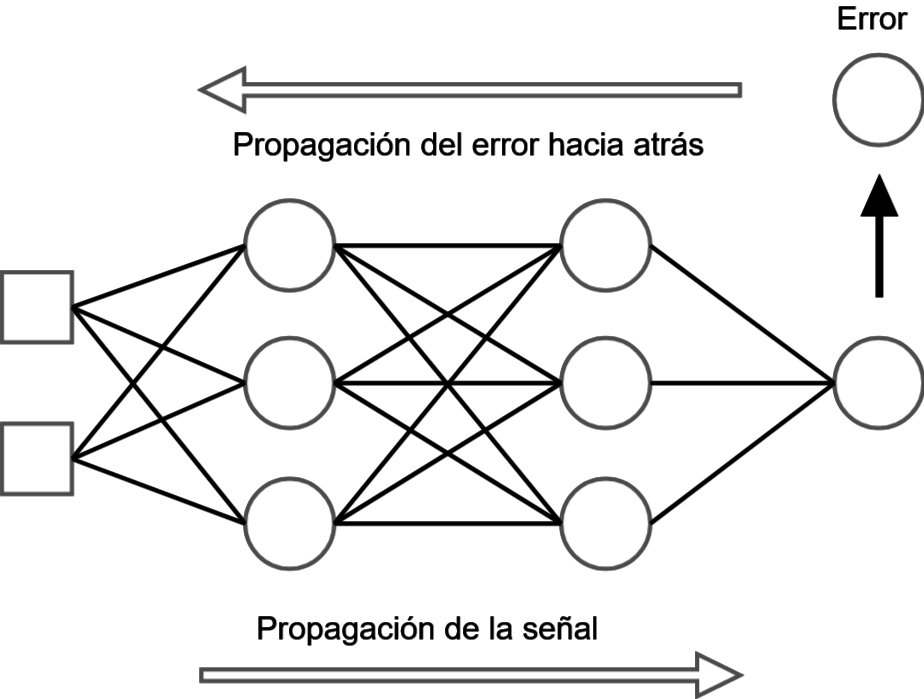
\includegraphics[width=0.8\textwidth]{MarcoTeorico/imgs/Backpropagation.png}
    \caption{Propagación hacia adelante y propagación hacia atrás.}
    \label{fig:backpropagation}
\end{figure}

\subsection{Descenso del Gradiente }

El método del descenso del gradiente es un algoritmo iterativo que minimiza una función de pérdida actualizando posteriormente los parámetros de la función.

\begin{figure}[H]
    \centering
    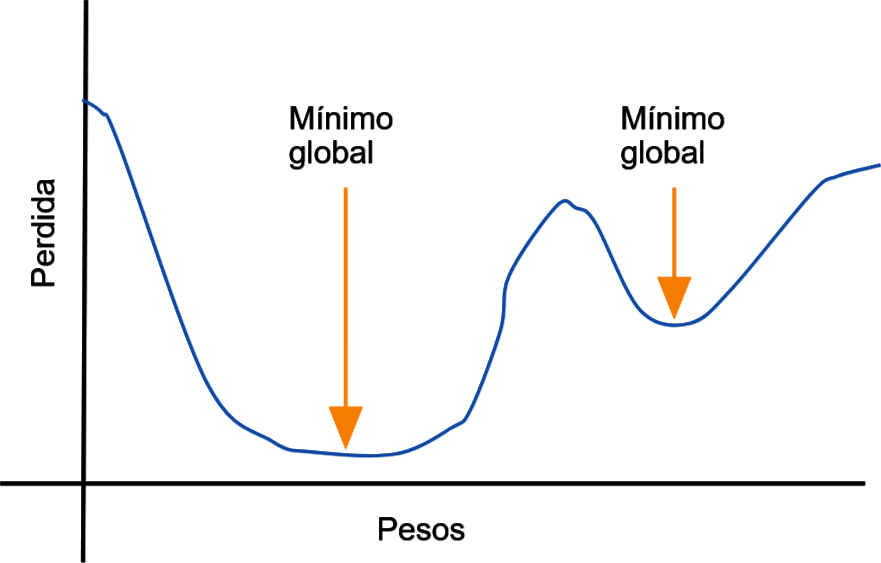
\includegraphics[width=0.7\textwidth]{MarcoTeorico/imgs/DescensoGradiente.png}
    \caption{Mínimo local y global.}
    \label{fig:descensoGradiente}
\end{figure}

La Figura \ref{fig:descensoGradiente} muestra cómo se puede tener múltiples picos y valles (Máximos y mínimos) para los valores de pérdida. El valor ideal que se desean obtener es el mínimo global, asegurando que los parámetros tomen los valores óptimos posibles.

El problema es que no se cuenta con una vista general en la que sea posible encontrar de manera sencilla el mínimo global ya que en realidad se inicializa en un lugar aleatorio sin saber dónde está el mínimo global y se avanza hacia una pérdida mínima sin subir accidentalmente a la cima de un máximo local.

\subsection{Tasa de aprendizaje}

La tasa de aprendizaje es uno de los hiperparámetros más importantes. Tiene un fuerte impacto tanto en la estabilidad como en la eficiencia de los tiempos de entrenamiento y no hay una forma fija de encontrar la más adecuada. La tasa de aprendizaje es la magnitud del ajuste de pesos durante el entrenamiento de la red con el fin de minimizar el error (\cite{valenzuela2020Sistema}).

La Figura \ref{fig:learningRate} muestra que, si la tasa es demasiado grande, el entrenamiento es inestable. Si la tasa de aprendizaje es demasiado pequeña, el entrenamiento puede tomar más tiempo para llegar al ideal.

\begin{figure}[H]
    \centering
    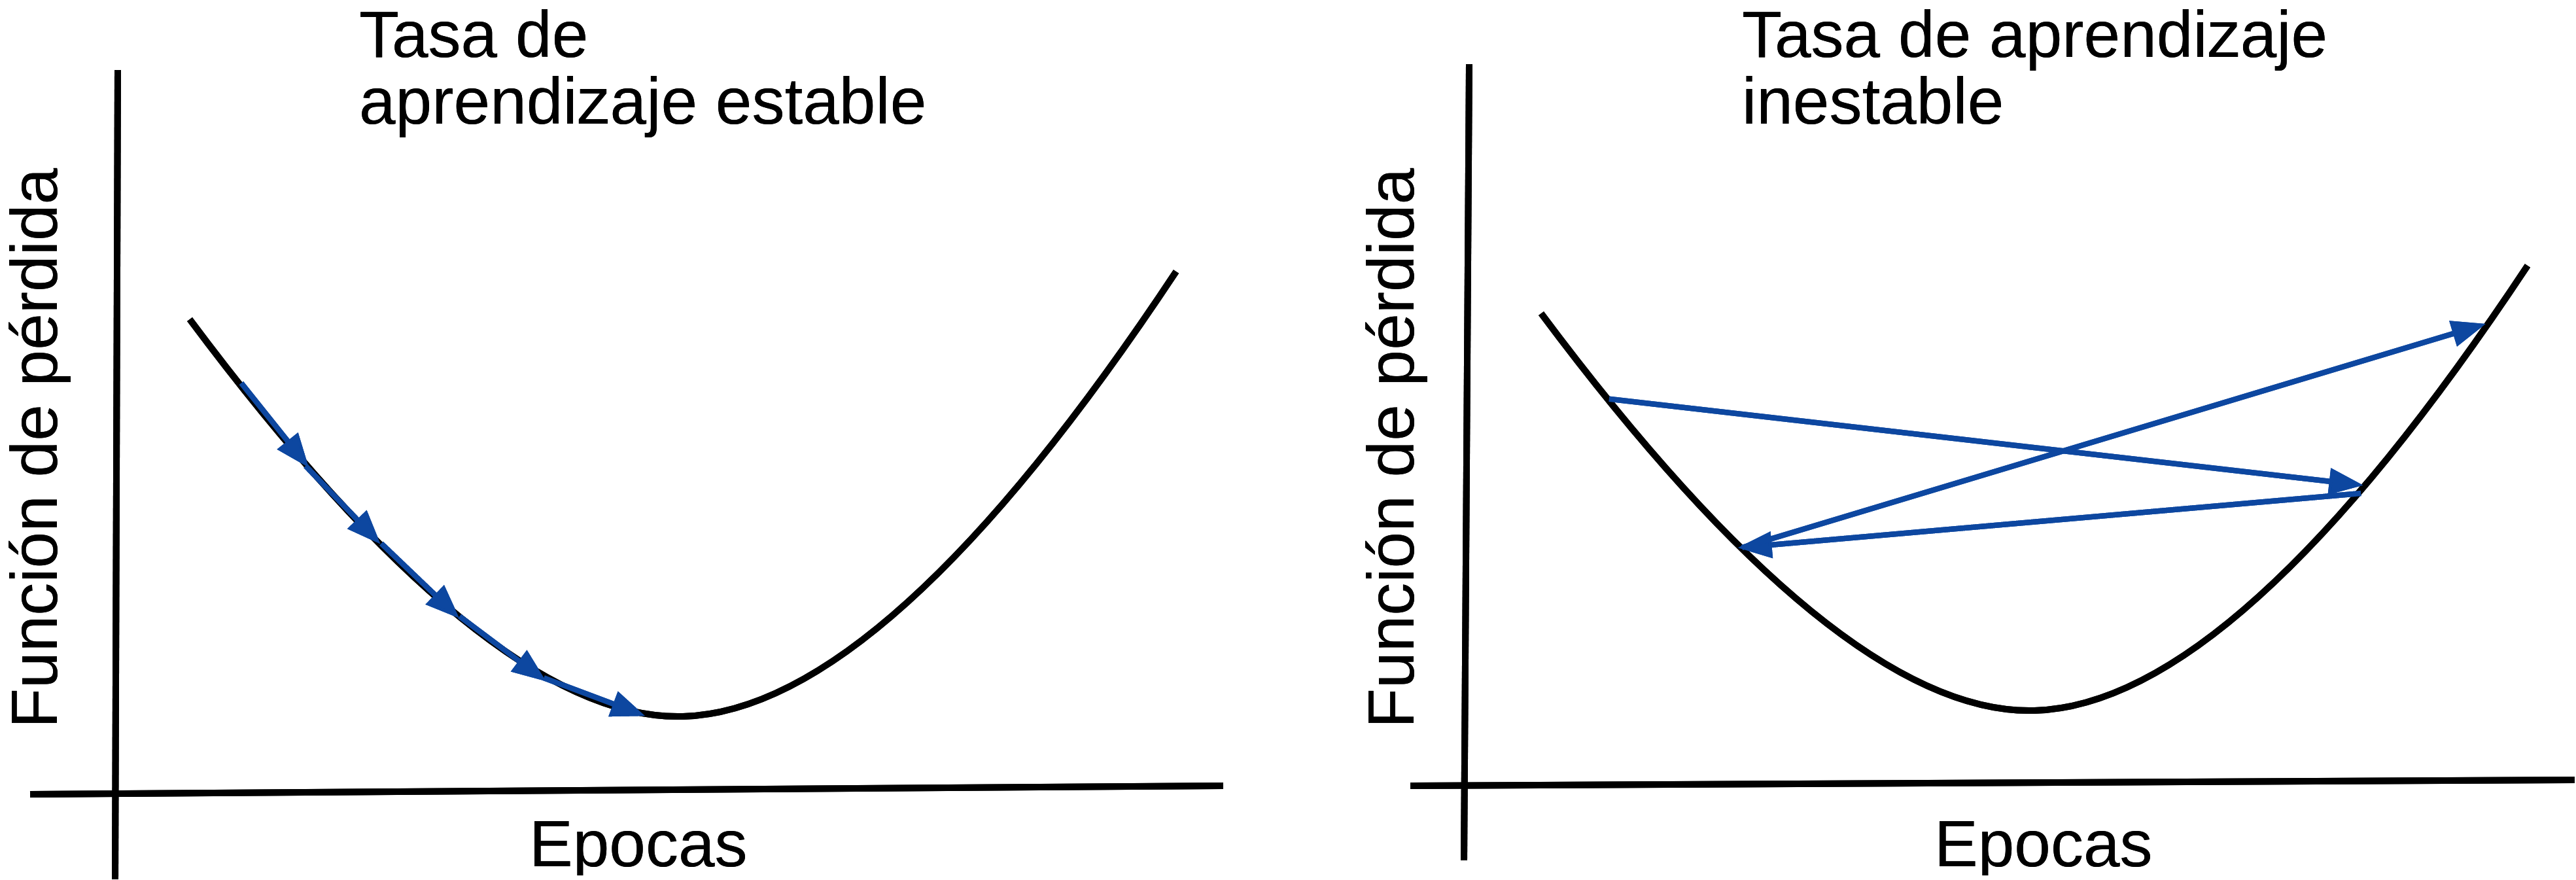
\includegraphics[width=0.8\textwidth]{MarcoTeorico/imgs/LearningRate.png}
    \caption{Tasa de aprendizaje.}
    \label{fig:learningRate}
\end{figure}

Preferiblemente, la pérdida de entrenamiento y validación casi se imitan entre sí, con solo una pequeña brecha entre la pérdida de entrenamiento y la pérdida de validación, lo que indica un pequeño sobreajuste. Siempre que la brecha no aumente drásticamente, existe un nivel aceptable de sobreajuste. Por otro lado, si no logra mantener esta brecha y las pérdidas de entrenamiento y validación se separan drásticamente, entonces se sabe que se corre el riesgo de sobreajuste. Una vez que la pérdida de validación comienza a aumentar, se sabe que estamos muy sobreajustados (\cite{rosebrock2017deep}).


\subsection{Funciones de activación}

Las funciones de activación son una función de escalar a escalar, que produce la activación de la neurona. Las funciones de activación son usadas para propagar la salida de los nodos de una capa hacia la siguiente capa y para que las neuronas ocultas en una red neuronal para introducir la no linealidad del modelado de la red (\cite{patterson2017deep}).


Las funciones de activación definen el rango de valores que dará como resultado una de las capas de nuestra red neuronal, a partir de una función matemática.

\subsubsection{Función lineal}

La función lineal regresa como salida valores en el rango de $[-\infty,\infty]$ y está dada por la Ecuación \ref{eq:linealFunc}:

\begin{equation}
\label{eq:linealFunc}
    f(x) = Wx
\end{equation}

La Figura \ref{fig:graficaLineal} muestra la gráfica generada por la Ecuación \ref{eq:linealFunc}.

\begin{figure}[H]
    \centering
    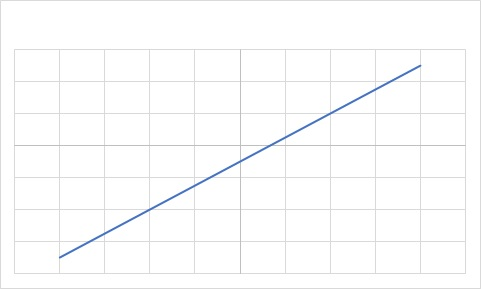
\includegraphics[width=0.5\textwidth]{MarcoTeorico/imgs/GraficaLineal.jpg}
    \caption{Gráfica de función lineal.}
    \label{fig:graficaLineal}
\end{figure}

\subsubsection{Sigmoidal}

La función sigmoidal tiene como salida valores en el rango de $[0,1]$ y está definida por la Ecuación \ref{eq:sigmoidFunc}:

\begin{equation}
\label{eq:sigmoidFunc}
    s(x)={\frac {1}{1+e^{-x}}}
\end{equation}

La Figura \ref{fig:graficaSigmoidal} muestra la gráfica generada por la Ecuación \ref{eq:sigmoidFunc}.

\begin{figure}[H]
    \centering
    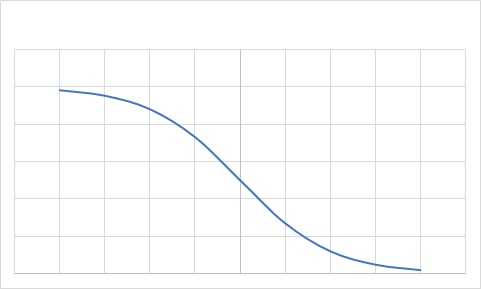
\includegraphics[width=0.5\textwidth]{MarcoTeorico/imgs/GraficaSigmoidal.jpg}
    \caption{Gráfica de función Sigmoidal.}
    \label{fig:graficaSigmoidal}
\end{figure}

\subsubsection{Tangente hiperbólica}

La función tangente hiperbólica proporciona como salida el rango $[-1,1]$ y está definida por la Ecuación \ref{eq:tanhFunc}.

\begin{equation}
\label{eq:tanhFunc}
    \tanh (x)={\cfrac {e^{x}-e^{-x}}{e^{x}+e^{-x}}}
\end{equation}

La Figura \ref{fig:graficaHiperbolica} muestra la gráfica generada por la Ecuación \ref{eq:tanhFunc}.

\begin{figure}[H]
    \centering
    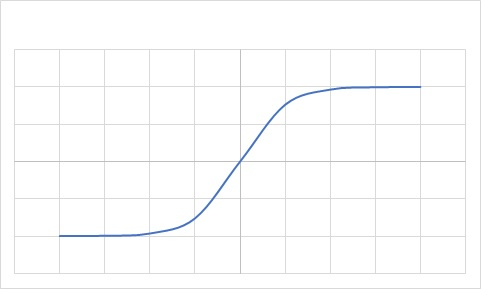
\includegraphics[width=0.5\textwidth]{MarcoTeorico/imgs/GraficaHiperbolica.jpg}
    \caption{Gráfica de función hiperbólica.}
    \label{fig:graficaHiperbolica}
\end{figure}

\subsubsection{Softmax}

La función de activación softmax devuelve la distribución de probabilidad sobre clases de salida mutuamente excluyentes. La cual está definida por la siguiente Ecuación \ref{eq:softmaxFunc}:

\begin{equation}
\label{eq:softmaxFunc}
  \sigma(\overrightarrow{z})_{i}=\frac{e^{z_{i}}}{
    \displaystyle\sum\limits_{j=1}^K e^{z_{j}}
  }
\end{equation}

donde $\overrightarrow{z}$ es el vector de entrada.

$z_i$ son los valores del vector de entrada, $e^{z_{i}}$ es la función exponencial estándar que se aplica a cada elemento del vector de entrada. $\displaystyle\sum\limits_{j=1}^K e^{z_{i}}$ es el término de normalización, asegura que todos los valores de salida de la función sumen 1 y cada uno esté en el rango $(0, 1)$, constituyendo así una distribución de probabilidad válida. Para finalmente, $k$ es el número de clases del clasificador multi-clases.

\subsubsection{ReLU}

La función Rectificador Lineal(ReLU) regresa como resultado valores en el rango de los números reales positivos $[0, \infty]$, como muestra la Ecuación \ref{eq:reluFunc}:

\begin{equation}
\label{eq:reluFunc}
  relu(x)=\max(0,x)
\end{equation}

La Figura \ref{fig:graficaReLU} muestra la gráfica generada por la Ecuación \ref{eq:reluFunc}.

\begin{figure}[H]
    \centering
    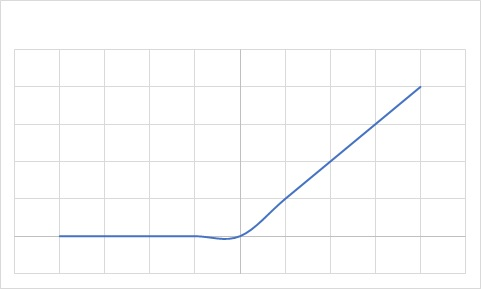
\includegraphics[width=0.5\textwidth]{MarcoTeorico/imgs/GraficaReLU.jpg}
    \caption{Gráfica de función ReLU.}
    \label{fig:graficaReLU}
\end{figure}

\subsection{Funciones de pérdida}

Una función de pérdida indica la pérdida de predicción de $\hat{y}$ cuando la salida real es $y$. El objetivo del entrenamiento es entonces minimizar la pérdida en los diferentes ejemplos de entrenamiento. La función asigna una puntuación numérica a la salida de la red $\hat{y}$ dada la verdadera salida esperada $y$ (\cite{goldberg2017Neural}).

Dependiendo del problema es el tipo de función de pérdida que se utiliza. Para un problema de regresión se busca tener la pérdida lo más cercana a cero y para un problema de clasificación se busca tener el valor más alto o muy cercano a 1 para cada una de las clases para la cual fue entrenada la red neuronal, siempre cuidando que la red neuronal no tenga sobreajuste.


Algunas de las funciones de pérdida para problemas de  regresión es el Error Cuadrático Medio (MSE, \textit{Mean squared error loss}) definido por la Ecuación \ref{eq:FPMSE} y el Error Absoluto Medio (MAE, \textit{Mean absolute error loss}) definido por la Ecuación \ref{eq:FPMAE}.

\begin{equation}
    \label{eq:FPMSE}
    MSE = (\frac{1}{n}) \displaystyle\sum\limits_{i=0}^n (y_i - x_i)^{2}
\end{equation}

\begin{equation}
    \label{eq:FPMAE}
    MAE = (\frac{1}{n}) \displaystyle\sum\limits_{i=0}^n \mid y_i - x_i \mid
\end{equation}

Mientras que para problemas de clasificación la pérdida de bisagra (\textit{Hinge loss}) es la función de pérdida mas común y definida por la Ecuación \ref{eq:FPHL}.

\begin{equation}
    \label{eq:FPHL}
    Hinge\: Loss = max(0, 1 – t)
\end{equation}


\subsection{Optimizadores}

Para el entrenamiento de una red neuronal es necesario adaptar los hiperparámetros de entrada para generar un buen modelo, en ocasiones suele ser una tarea complicada ya que no hay un manual que indique como configurar los hiperparámetros de tal manera que el modelo proporcione los mejores resultados, por lo tanto, es una tarea de prueba y error.

La tasa de aprendizaje suele ser uno de los hiperparámetros más relevantes afectando directamente en el tiempo de entrenamiento de la red. Con ayuda del descenso del gradiente, este hiperparámetro puede resultar de mucha ayuda para el entrenamiento, sin embargo, tiene la limitante de que la tasa de aprendizaje es un valor fijo, por otra parte, existen algoritmos que ayudan a reducir el valor de la tasa de aprendizaje para mejorar los resultados del modelo.

Los optimizadores adaptativos son mejoras al algoritmo del descenso de gradiente los cuales cambian el valor de la tasa de aprendizaje para cada parámetro, tomando como referencia los resultados obtenidos. Algunos de los optimizadores más populares son los siguientes:

\begin{itemize}
    \item AdaGrad (\textit{Adaptative Gradient Algorithm}): Este algoritmo se encarga de modificar el valor de la taza de aprendizaje para mejorar los resultados y el tiempo de entrenamiento.
    \item AdaDelta: Es una extensión de AdaGrad para reducir el cambio drástico de la tasa de aprendizaje.
    \item RMSProp (\textit{Root Mean Squared Propagation}): Al igual que AdaDelta, RMSProp ayuda a reducir el cambio drástico de la tasa de aprendizaje del AdaGrad.
\end{itemize}
